% Figure 1: the epistemic hierarchy (left) and the minimal production loop (right)
\documentclass[tikz,border=8pt]{standalone}
% Shared preamble for SAI taxonomy standalone figures.
% Self-contained: no MetaCircle dependency; colors match the paper palette.
\usepackage{amsmath,amssymb}
\usetikzlibrary{arrows.meta}
\definecolor{MetaPurple}{HTML}{6D3BD1}
\definecolor{MetaViolet}{HTML}{9B5DE5}
\definecolor{MetaCoral}{HTML}{D76A7A}
\definecolor{MetaInk}{HTML}{16131D}
\definecolor{MetaGray}{HTML}{F4F2F7}
\definecolor{MetaMidGray}{HTML}{6E6875}
\newcommand{\Lk}{\mathcal{L}_1}
\newcommand{\Ll}{\mathcal{L}_2}
\newcommand{\Ls}{\mathcal{L}_3}
\newcommand{\Op}[1]{\textsc{#1}}
\newcommand{\universe}{\Omega}
\newcommand{\kb}{\mathcal{K}}
\newcommand{\cell}{\omega}

\begin{document}
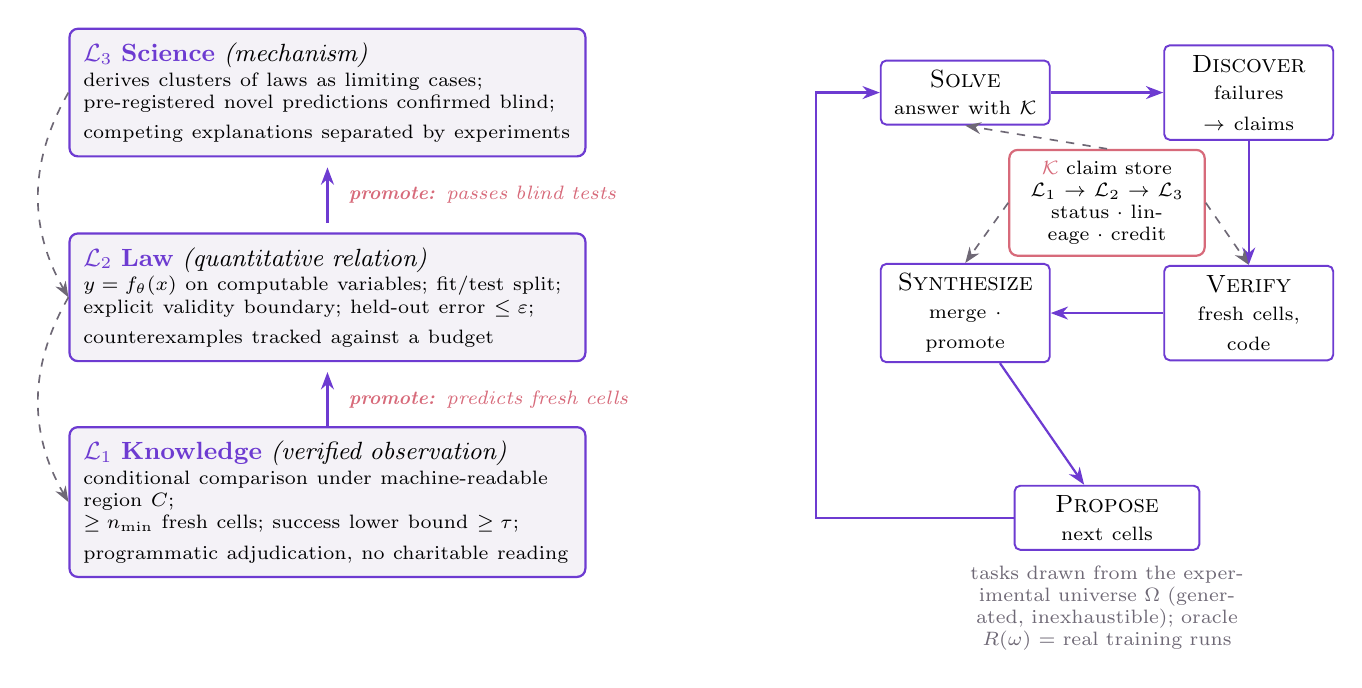
\begin{tikzpicture}[
  font=\small,
  lvl/.style={draw=MetaPurple, rounded corners=3pt, align=left, inner sep=5pt, fill=MetaGray, line width=0.8pt},
  gate/.style={font=\scriptsize\itshape, text=MetaCoral, align=left},
  op/.style={draw=MetaPurple, rounded corners=2pt, align=center, inner sep=3.5pt, fill=white, line width=0.7pt, minimum height=7mm, font=\small},
  ar/.style={-{Stealth[length=2.2mm]}, line width=0.8pt, MetaPurple},
  ard/.style={-{Stealth[length=2mm]}, line width=0.6pt, MetaMidGray, dashed},
]
% ---------------- left panel: the ladder ----------------
\node[lvl, text width=6.2cm] (L3) at (0,5.2) {%
  \textbf{\textcolor{MetaPurple}{$\mathcal{L}_3$ Science}} \emph{(mechanism)}\\[1pt]
  \scriptsize derives clusters of laws as limiting cases;\\
  \scriptsize pre-registered novel predictions confirmed blind;\\
  \scriptsize competing explanations separated by experiments};
\node[lvl, text width=6.2cm] (L2) at (0,2.6) {%
  \textbf{\textcolor{MetaPurple}{$\mathcal{L}_2$ Law}} \emph{(quantitative relation)}\\[1pt]
  \scriptsize $y = f_\theta(x)$ on computable variables; fit/test split;\\
  \scriptsize explicit validity boundary; held-out error $\leq \varepsilon$;\\
  \scriptsize counterexamples tracked against a budget};
\node[lvl, text width=6.2cm] (L1) at (0,0) {%
  \textbf{\textcolor{MetaPurple}{$\mathcal{L}_1$ Knowledge}} \emph{(verified observation)}\\[1pt]
  \scriptsize conditional comparison under machine-readable region $C$;\\
  \scriptsize $\geq n_{\min}$ fresh cells; success lower bound $\geq \tau$;\\
  \scriptsize programmatic adjudication, no charitable reading};
% promote arrows (center) with gate labels in the gaps
\draw[ar] (0,0.95) -- node[gate, right=4pt, text width=4.3cm]{\textbf{promote:} predicts fresh cells} (0,1.65);
\draw[ar] (0,3.55) -- node[gate, right=4pt, text width=4.3cm]{\textbf{promote:} passes blind tests} (0,4.25);
% demote arrows (bowed left)
\draw[ard] (L2.west) to[bend right=30] (L1.west);
\draw[ard] (L3.west) to[bend right=30] (L2.west);

% ---------------- right panel: the minimal loop ----------------
\begin{scope}[shift={(8.1,0)}]
  \node[op, text width=1.9cm] (solve) at (0,5.2) {\Op{Solve}\\[-1pt]\scriptsize answer with $\mathcal{K}$};
  \node[op, text width=1.9cm] (disc) at (3.6,5.2) {\Op{Discover}\\[-1pt]\scriptsize failures $\to$ claims};
  \node[op, text width=1.9cm] (ver) at (3.6,2.4) {\Op{Verify}\\[-1pt]\scriptsize fresh cells, code};
  \node[op, text width=1.9cm] (syn) at (0,2.4) {\Op{Synthesize}\\[-1pt]\scriptsize merge $\cdot$ promote};
  \node[op, text width=2.1cm] (prop) at (1.8,-0.2) {\Op{Propose}\\[-1pt]\scriptsize next cells};
  \node[draw=MetaCoral, rounded corners=3pt, align=center, inner sep=4pt, text width=2.2cm, font=\scriptsize, line width=0.8pt] (kb) at (1.8,3.8) {\textbf{\textcolor{MetaCoral}{$\mathcal{K}$}} claim store\\ $\mathcal{L}_1 \to \mathcal{L}_2 \to \mathcal{L}_3$\\ status $\cdot$ lineage $\cdot$ credit};
  \draw[ar] (solve) -- (disc);
  \draw[ar] (disc) -- (ver);
  \draw[ar] (ver) -- (syn);
  \draw[ar] (syn) -- (prop);
  \draw[ar] (prop.west) -- (-1.9,-0.2) |- (solve.west);
  \draw[ard] (kb.north) -- (solve.south);
  \draw[ard] (kb.east) -- (ver.north);
  \draw[ard] (kb.west) -- (syn.north);
  \node[font=\scriptsize, text=MetaMidGray, align=center, text width=4.3cm] at (1.8,-1.35) {tasks drawn from the experimental universe $\Omega$ (generated, inexhaustible); oracle $R(\omega)$ = real training runs};
\end{scope}
\end{tikzpicture}
\end{document}
